\documentclass[12pt]{article}
\usepackage{amsmath}
\usepackage{graphicx}
\usepackage{hyperref}
\usepackage[utf8]{inputenc}
\usepackage[spanish]{babel}
\usepackage[margin=3cm]{geometry}
\usepackage{amsfonts}
\usepackage{listings}
\usepackage[T1]{fontenc}
\usepackage{float}
\usepackage{subfig}

\title{Practica 2 - Visión por Computador.}
\author{Néstor Rodríguez Vico. DNI: 75573052C - \href{mailto:nrv23@correo.ugr.es}{nrv23@correo.ugr.es}}
\date{\today}


\lstdefinestyle{bash_style}{
	language=bash,
	frame=single,
	xleftmargin=.25in,
	upquote = true,
	basicstyle=\scriptsize,
	breakatwhitespace=false,         
	breaklines=true,                 
	captionpos=b,                    
	keepspaces=true,                 
	numbers=left,                    
	numbersep=5pt,                  
	showspaces=false,                
	showstringspaces=false,
	showtabs=false,                  
	tabsize=2
}

\lstset{style=bash_style}

\begin{document}
\maketitle

\setlength{\belowdisplayskip}{5pt} 
\setlength{\belowdisplayshortskip}{5pt}
\setlength{\abovedisplayskip}{5pt} 
\setlength{\abovedisplayshortskip}{5pt}

\section{Chroma Key.}

A continuación se muestra el resultado del chroma key. La idea aplicada está en los comentarios del código. En la primera imagen se muestra el resultado sin ningún desplazamiento. En la segunda, se desplaza la imagen de la mujer para que coincida con la parte baja de la imagen de fondo:

\begin{table}[H]
	\centering
	\begin{tabular}{cc}
		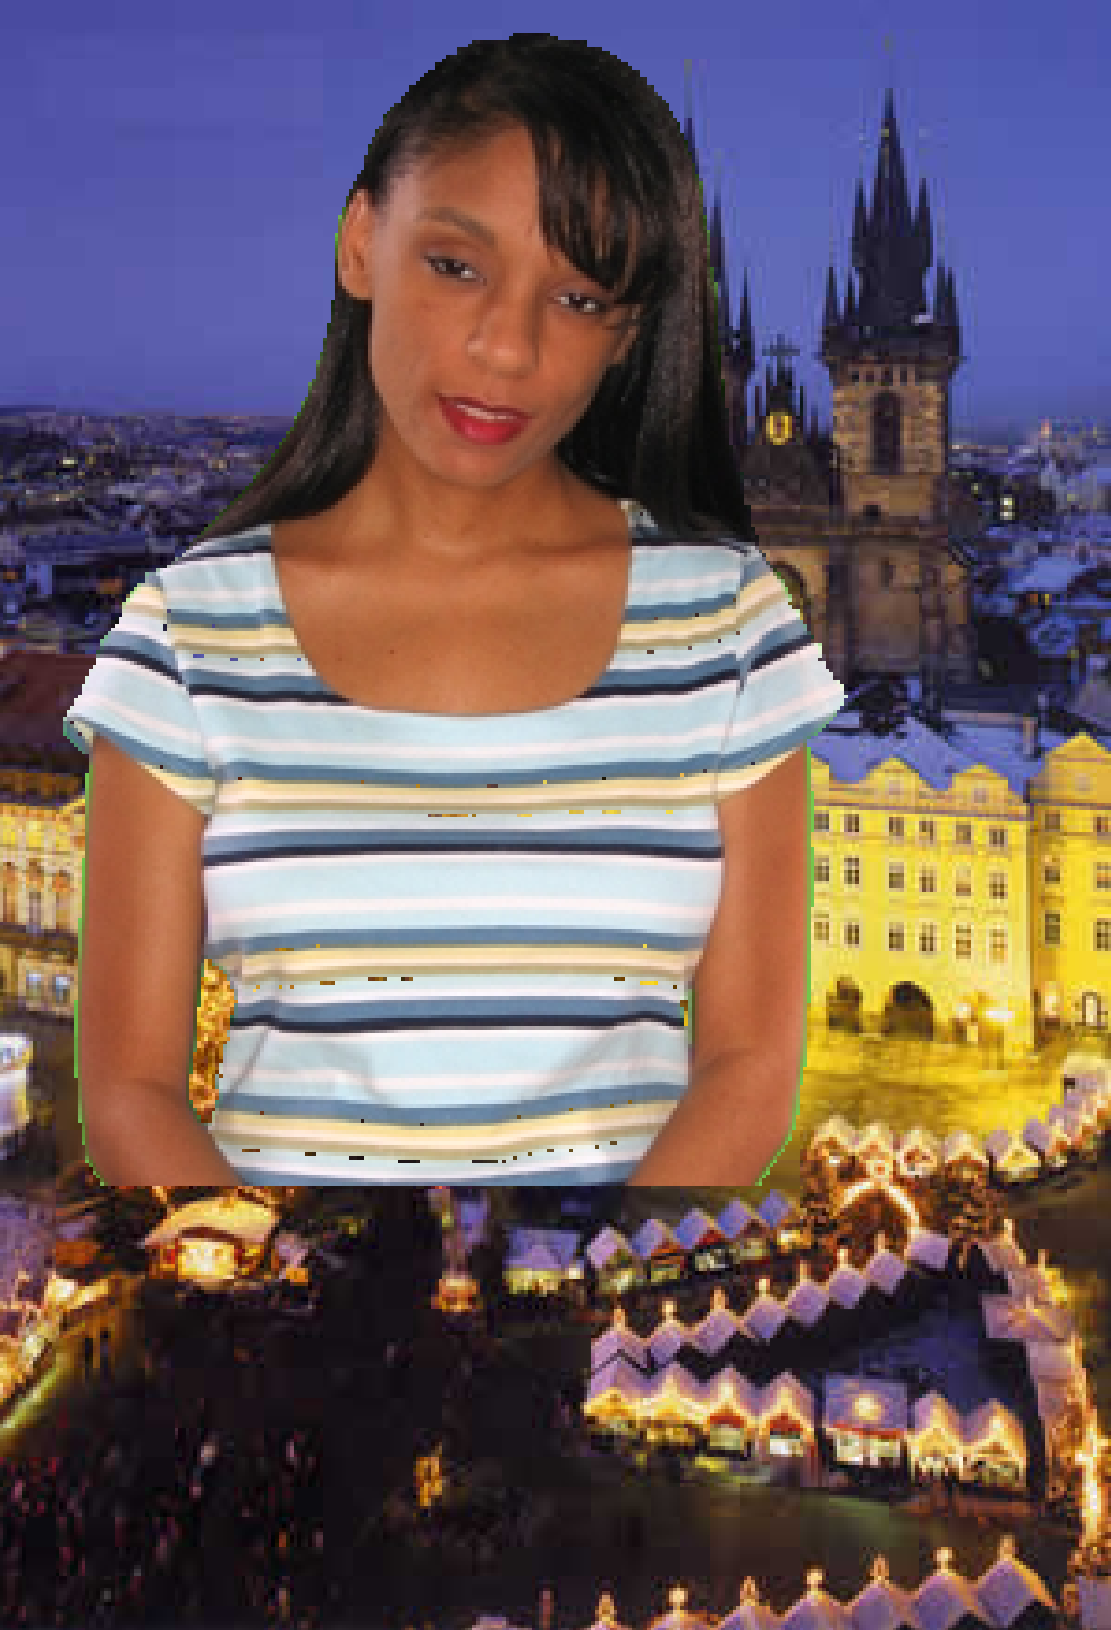
\includegraphics[width=0.4\linewidth]{images/1.png} &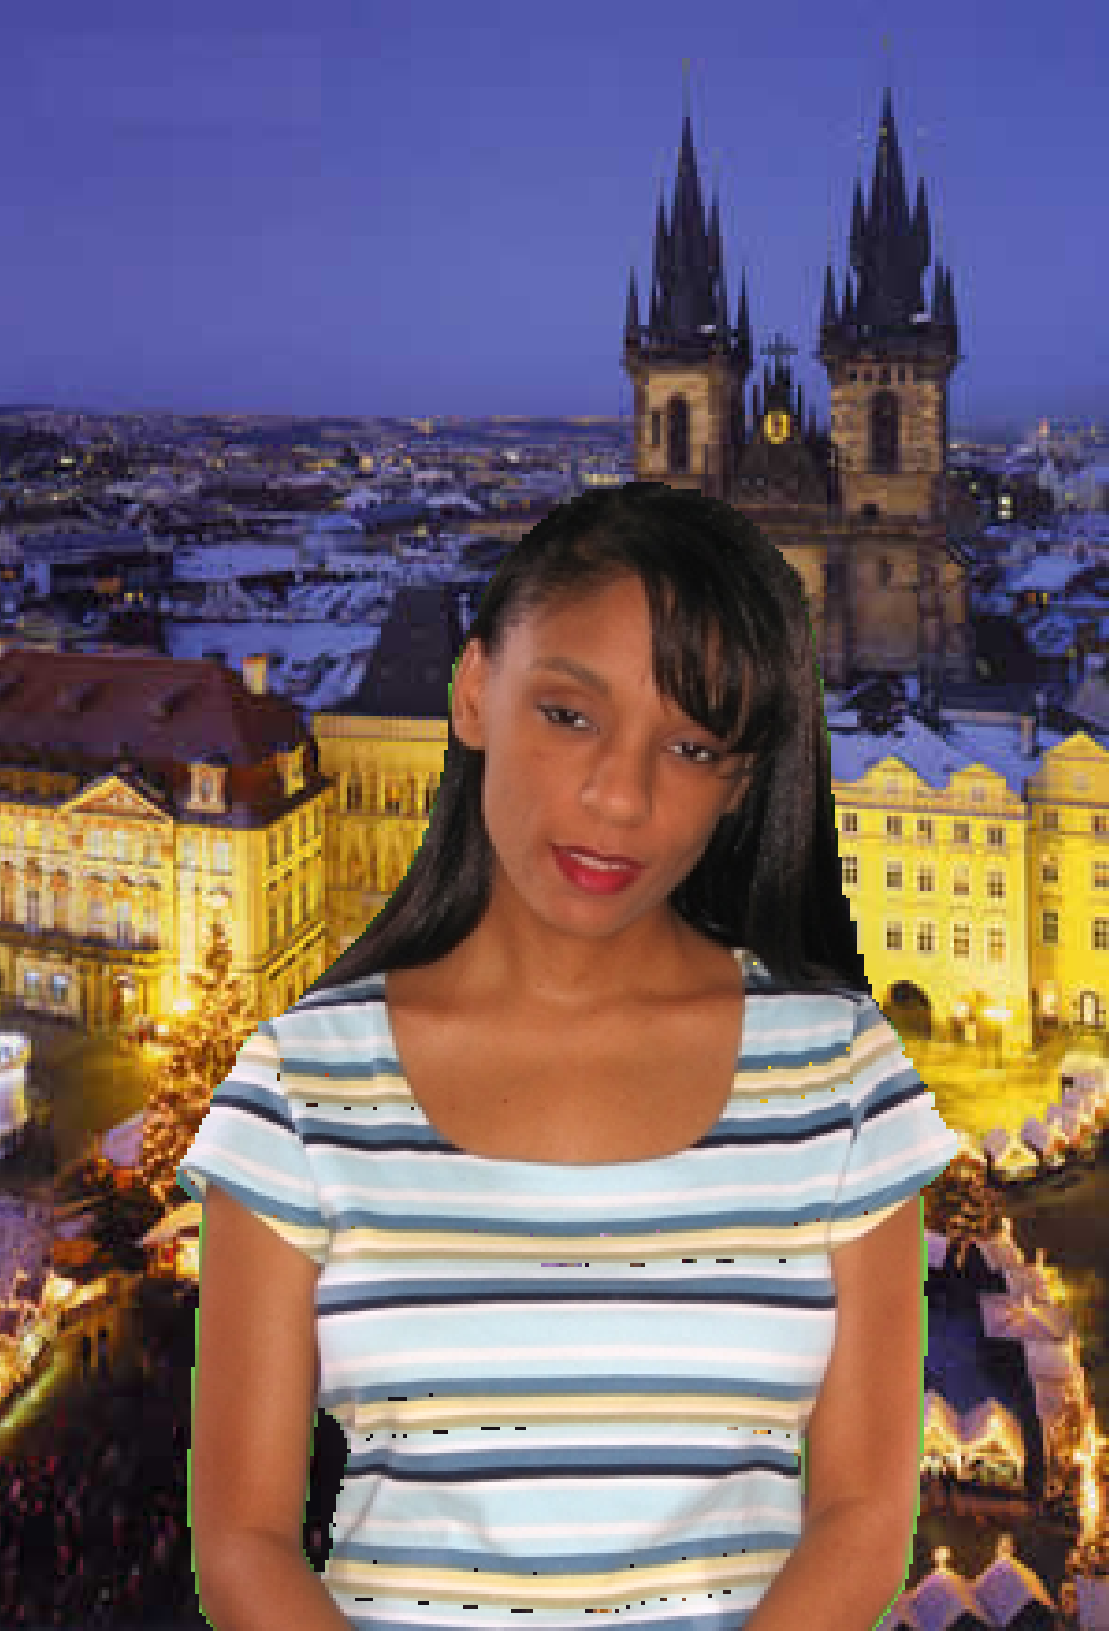
\includegraphics[width=0.4\linewidth]{images/2.png}
	\end{tabular}
\end{table}



\end{document}